\documentclass{beamer}

\usepackage{amssymb,amsmath}
\usepackage{graphicx}
\usepackage{url}
\usepackage{color}
\usepackage{pagenote}[continuous,page]
\usepackage{relsize}		% For \smaller
\usepackage{url}			% For \url
\usepackage{epstopdf}	% Included EPS files automatically converted to PDF to include with pdflatex

%For MindMaps
% \usepackage{tikz}%
% \usetikzlibrary{mindmap,trees,arrows}%

%%% Color Definitions %%%%%%%%%%%%%%%%%%%%%%%%%%%%%%%%%%%%%%%%%%%%%%%%%%%%%%%%%
%\definecolor{bordercol}{RGB}{40,40,40}
%\definecolor{headercol1}{RGB}{186,215,230}
%\definecolor{headercol2}{RGB}{80,80,80}
%\definecolor{headerfontcol}{RGB}{0,0,0}
%\definecolor{boxcolor}{RGB}{186,215,230}

%%% Save space in lists. Use this after the opening of the list %%%%%%%%%%%%%%%%
%\newcommand{\compresslist}{
%	\setlength{\itemsep}{1pt}
%	\setlength{\parskip}{0pt}
%	\setlength{\parsep}{0pt}
%}

%\setbeameroption{show notes on top}

% You should run 'pdflatex' TWICE, because of TOC issues.

% Rename this file.  A common temptation for first-time slide makers
% is to name it something like ``my_talk.tex'' or
% ``john_doe_talk.tex'' or even ``discrete_math_seminar_talk.tex''.
% You really won't like any of these titles the second time you give a
% talk.  Try naming your tex file something more descriptive, like
% ``riemann_hypothesis_short_proof_talk.tex''.  Even better (in case
% you recycle 99% of a talk, but still want to change a little, and
% retain copies of each), how about
% ``riemann_hypothesis_short_proof_MIT-Colloquium.2000-01-01.tex''?

\mode<presentation>
{
  \usetheme{CambridgeUS}		% bem bacana - menu superior
  \usecolortheme{default}		% branco, azul clarinho
  \useoutertheme{default}
  \useinnertheme{circles}
  \setbeamercovered{invisible}
}

\beamertemplatenavigationsymbolsempty

%% Better looking blocks
\setbeamercolor{block title alerted}{use=structure,fg=black,bg=red!80!black}
\setbeamercolor{block body alerted}{use=structure,fg=black,bg=white!90!black}

\setbeamercolor{block title}{use=structure,fg=black,bg=blue!60!white}
\setbeamercolor{block body}{use=structure,fg=black,bg=white!90!black}

\usepackage[english]{babel}
\usepackage[latin1]{inputenc}
\usepackage{subfigure}

\usepackage{times}
\usepackage[T1]{fontenc}

%% makes the ppagenote command for figure references at the end.
\makepagenote
\renewcommand{\notenumintext}[1]{}
\newcommand{\ppagenote}[1]{\pagenote[Page \insertframenumber]{#1}}


\title[GB13604]{GB13604 - Maths for Computer Science}
\subtitle[]{Lecture 2 -- Proofs, Part 2}
\author[Claus Aranha]{Claus Aranha\\{\footnotesize caranha@cs.tsukuba.ac.jp}}
\institute[COINS]{College of Information Science}
\date[2018-10-10]{2018-10-10\\{\tiny Last updated \today}}

\begin{document}


\begin{frame}
  \maketitle

  \begin{center}
    {\smaller This course is based on Mathematics for Computer Science, Spring
    2015, by Albert Meyer and Adam Chlipala, Massachusetts Institute
    of Technology OpenCourseWare.}
    
    
\includegraphics[width=0.2\textwidth]{../img/by-nc-sa}
  \end{center}
\end{frame}

\section{Introduction}

\subsection{In the last class}
\begin{frame}
  \frametitle{Last Class Review}

  {\huge
  \begin{itemize}
  \item Proofs
    \begin{itemize}
      {\huge
      \item Proof by Contradiction
      \item Proof by Cases
      }
    \end{itemize}
  \item The Well Ordered Principle
  \item Predicate Satisfiability (SAT)
  \item Predicate Validity
  \end{itemize}
  }
\end{frame}

\begin{frame}
  \frametitle{Exercise Discussion}
\end{frame}

\begin{frame}
  \frametitle{For This Lecture...}

  {\larger
  
  Textbook Chapters 4,5,6 (and a bit of 7)
  
  \bigskip
  
  \begin{itemize}
  \item Sets
  \item \alert{Induction}
  \item State Machines
  \end{itemize}

  }
\end{frame}

\section{Sets}
\subsection{Definition of sets}

\begin{frame}
  
  \begin{center}
    {\larger
      Mathematical Data Structures

      \bigskip
      
      The Set
    }
  \end{center}
\end{frame}

\begin{frame}
  \frametitle{Definition of Set}

  {\larger
  \begin{itemize}
  \item The most fundamental of mathematical data types;
  \item A \alert{collection} of mathematical objects
    \begin{itemize}
    \item ... circular definition: what is a collection?
    \end{itemize}
  \end{itemize}

  \vfill

  Examples:
  \begin{itemize}
  \item Real Numbers $\mathbb{R}$,
  \item Complex numbers $\mathbb{C}$,
  \item Empty Set $\varnothing$
  \end{itemize}  
  }
\end{frame}

\begin{frame}
  \frametitle{More examples of Sets}

  {\larger
    \begin{itemize}
    \item \{7, ``Aranha'', $\pi/2$, TRUE\}
    \item \{TRUE, 7, $\pi/2$, ``Aranha''\}
    \item \{7, $\pi$\} = \{7, $\pi$, 7\}
    \end{itemize}

    \vfill

    \begin{itemize}
    \item Mathematical sets can mix different ``types''
    \item Mathematical sets do not care about ``order''
    \item Mathematical sets do not have duplicates.
    \end{itemize}
  }
\end{frame}

\begin{frame}
  \frametitle{Set Membership}

  {\larger
  The most fundamental property of a set is \structure{membership}.

  \bigskip

  \begin{itemize}
  \item A = \{7,TRUE,$\pi$\}
  \item $7 \in A$
  \item 7 is an element of $A$,
  \item $3 \notin A$

    \vfill

  \item $7 \in \mathbb{Z}$
  \item $\mathbb{Z} \in \{3, \mathbb{Z}, 7\}$
  \item A set can be a member of another set.    
  \end{itemize}
  }
\end{frame}

\begin{frame}
  \frametitle{Definition of Subset}
  {\larger
  \begin{block}{Subset}
    \begin{itemize}
    \item $A \subset B$ means that every element of A is also an element of B
    \item $A\subset B \text{ equiv }\forall x, x\in A \rightarrow x\in B$
    \item $\mathbb{Z} \subset \mathbb{R}, \mathbb{R} \subset \mathbb{C}, \{3\} \subset \{5,3,7\}$
    \end{itemize}
  \end{block}

  \begin{block}{Important!}
    \begin{itemize}
    \item $A \subset A$
    \item $\forall X\text{ is a set}, \varnothing \subset X$
    \end{itemize}
  \end{block}
  }
\end{frame}

\begin{frame}
  \frametitle{Difference between Membership and Subset}

  {\huge
  \begin{itemize}
  \item $3 \in \{3,5,6\}$
  \item $3 \not\subset \{3,5,6\}$
  \end{itemize}

  \vfill

  \begin{itemize}
  \item $\{3\} \subset \{3,5,6\}$
  \item $\{3\} \notin \{3,5,6\}$
  \end{itemize}
  }
\end{frame}

\begin{frame}
  \frametitle{Prove that the empty set subsets everything}

  {\larger
  \begin{enumerate}
  \item $A \subset B$ means that $\forall x, x \in A \rightarrow x \in B$
    \bigskip
    
  \item If $A = \varnothing$ then $x \in A$ is FALSE for $\forall x$
    \bigskip
    
  \item Replace ``$\forall x \in A$'' with FALSE
    \bigskip
    
  \item FALSE $\rightarrow x \in B$ is always TRUE. \\(FALSE $\rightarrow X$ is always TRUE)
    \bigskip
    
  \item Therefore, $\varnothing \subset B$ is TRUE $\forall B$    
  \end{enumerate}
  }
\end{frame}

\begin{frame}
  \frametitle{Predicate Definition of Set Membership}

  In many cases, we use a predicate to determine membership in a
  set. Let $P(X)$ be a predicate that defines set $A$. If $P(X)$ is
  true for a certain $X$, then $X \in A$.

  \begin{block}{Example 1}
    \begin{itemize}
    \item $A = x \in \mathbb{N}, \{x < 12 \text{ AND } x \text{ is prime}\}$
    \item $A = \{2,3,5,7,11\}$
    \end{itemize}    
  \end{block}
  
  \begin{block}{Example 2}
    \begin{itemize}
    \item $B = x \in \mathbb{N}, \{x \text{ is prime AND } x+2 \text{ is prime}\}$
    \item $B = \{3 (5), 5 (7), 11 (13), 17 (19), 29 (31), \ldots\}$
    \end{itemize}
  \end{block}
\end{frame}

\begin{frame}
  \frametitle{The Power Set}
  The Power set of A is a special set composed of ALL subsets of A.

  \begin{equation*}
    POW(A) = \forall x \subset A, x \in POW(A)
  \end{equation*}

  For example:

  \begin{equation*}
    POW(\{T,F\}) = \{\{T\},\{F\},\{T,F\},\varnothing\}
  \end{equation*}

  Also:

  \begin{equation*}
    \mathbb{N} \in POW(\mathbb{R}), \mathbb{N} \subset \mathbb{R}, \mathbb{N} \notin \mathbb{R}
  \end{equation*}
\end{frame}

\subsection{Operations on Sets}

\begin{frame}
  \frametitle{Operations on Sets}

  {\larger
    We can use operations on sets to create new sets:
    \begin{itemize}
    \item Union: $A \cup B \rightarrow x \in A \lor x \in B$
    \item Intersection: $A \cap B \rightarrow x \in A \land x \in B$
    \end{itemize}

    \bigskip
    
    Union and intersection are \structure{distributive}:
    \begin{equation*}
      A \cup (B \cap C) = (A \cup B) \cap (A \cup C)
    \end{equation*}
    Let's prove this.

  }
\end{frame}

\begin{frame}
  \frametitle{Proof: $A \cup (B \cap C) = (A\cup B)\cap(A\cup C)$}
  {\larger
    {\bf We prove this by a sequence of IFF.}\\
    \begin{enumerate}
    \item $x \in A \cup (B \cap C)$ {\bf iff}
    \item $x \in A \lor x \in (B \cap C)$ {\bf iff} \hfill (definition of union)
    \item $x \in A \lor (x \in B \land x \in C)$ {\bf iff} \hfill
      (definition of intersection)
    \item $(x \in A \lor x \in B) \land (x\in A \lor x \in C)$ {\bf
      iff} \hfill (distributive prop.)
    \item $(x \in A\cup B) \land (x \in A\cup C)$ {\bf iff}\hfill
      (definition of union)
    \item $x \in (A\cup B)\cap (A\cup C)$ {\bf done.} \hfill
      (fefintion of intersection)
      
    \end{enumerate}
  }
\end{frame}

\begin{frame}
  \frametitle{Set Subtraction and Complement}

  {\larger
    \begin{itemize}
    \item Subtraction: $A - B \rightarrow x \in A \land x \notin B$

      \bigskip
      
    \item Complement: $\overline{A} = D - A$, where $D$ is the domain.
    \end{itemize}
  }             
\end{frame}

\section{Binary Relations}
\begin{frame}
  \begin{center}
    {\huge
      Binary Relations
    }
  \end{center}
\end{frame}


\subsection{Binary Relations}
\begin{frame}
  \frametitle{Relations and Functions}

  {\larger
    \begin{itemize}
    \item Functions are a special case of \structure{binary relations}
    \item Binary relations associate the elements of one set
      (\alert{the domain}), with the elements of another set
      (\alert{the co-domain})

      \vfill

    \item We discussed this when talking about membership in sets
      (from $\mathbb{N}$ to the set of Even numbers).
    \item We also see relations in: Relational Databases (SQL, mySQL),
      counting the size of sets, and theory of computing.
    \end{itemize}
  }
\end{frame}

\begin{frame}
  \frametitle{Initial Example}

  {\larger
    Consider the relation \structure{Student Registered for Course} -- {\bf R}

    \begin{center}
      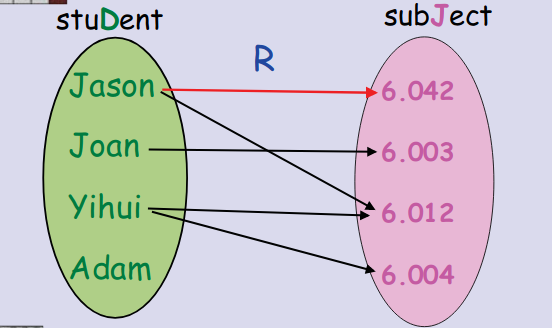
\includegraphics[width=0.8\textwidth]{../img/relations}
    \end{center}

    Why is this different than a function?
  }
\end{frame}

\begin{frame}
  \frametitle{{\bf R} -- Student Registered for Course}

  {\larger
    Components of the relation:
    \begin{itemize}
    \item Domain: List of Students;
    \item Co-domain: List of Classes;
    \item Relation Graph: List of ``arrows'' linking students and courses.      
      
      \bigskip

    \item R(Jason) = $\{6.042, 6.012\}$
    \item Jason R 6.042
    \item $R(\{Jason, Yihui\}) = \{6.042, 6.012, 6.004\}$
    \end{itemize}
  }
\end{frame}

\begin{frame}
  \frametitle{Relations and Inverse Relations}

  {\larger
    Relation:
    \begin{equation*}
      R(X) ::= {j \in J | \exists d \in X. d R j}
    \end{equation*}

    \bigskip
    Reverse Relation:
    \begin{equation*}
      R^{-1}(Y) ::= {d \in S | \exists j \in Y. d R j}
    \end{equation*}

    \bigskip

    \begin{itemize}
    \item $R(Jason) = \{6.042, 6.012\}$
    \item $R^{-1}(6.012) = \{Jason, Yihui\}$
    \end{itemize}
  }
\end{frame}

\subsection{Composing Relations}

\begin{frame}
  \frametitle{Composite Relations}

  {\larger Let's imagine a second relation between
    \structure{professors} and \structure{students}.
  }
  \begin{center}
    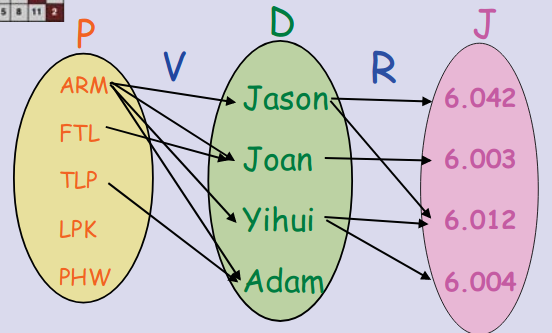
\includegraphics[width=0.8\textwidth]{../img/composite_relation}
  \end{center}
\end{frame}

\begin{frame}
  \frametitle{Composite Relations}

  {\large
    We can define the relation {\bf V} in the same way that we defined {\bf R}.

    \bigskip

    But we can also compose the two relations, {\bf V and R}, to get
    the set of courses that a professor's students are enrolled:
    \begin{itemize}
    \item $R(V(X))$ or $(R\circ V)(X)$
    \item $R(V(FTL)) = \{6.003\}$ 
    \end{itemize}
  }
\end{frame}

% TODO: Add a discussion about a relation T (teaching) and its relation
% with RV (for example, can we test whether T\intRV = nothing?)

\begin{frame}
  \frametitle{Binary Relations}

  {\larger We can classify relations depending on the number of
    ``arrows'' coming out of the domain, or coming in to the
    co-domain.

    \bigskip

    Classification based on the Domain
    \begin{itemize}
    \item {\bf Total Relation}: Every element has $\geq 1$ out arrows.
    \item {\bf Function}: Every element has $\leq 1$ out arrows.
    \end{itemize}

    Classification based on the Co-Domain
    \begin{itemize}
    \item {\bf Surjection}: Every element has $\geq 1$ in arrows
    \item {\bf Injection}: Every element has $\leq 1$ in arrows
    \end{itemize}

    \bigskip
    Finally:
    \begin{itemize}
    \item {\bf Bijection}: A relation is a {\bf surjection function}
    \end{itemize}    
  }
\end{frame}

\begin{frame}
  \frametitle{Binary Relations: Example}

  {\larger
    \begin{block}{$g: \mathbb{R}\times\mathbb{R} \rightarrow \mathbb{R}. g(x,y) = 1/(x-y)$}
      \begin{itemize}
      \item This is a {\bf function} (each x,y has only one output)
      \item This is not a {\bf total function} (g(x=y) is not defined)
      \end{itemize}      
    \end{block}

    \begin{block}{$g_o: \mathbb{R}^2 - \{x,y|x=y\} \rightarrow \mathbb{R}. g_o(x,y) = 1/x-y)$}
      \begin{itemize}
      \item $g_o$ has the same graph (arrows) as $g$, but different domain.
      \item $g_o$ is a total function.
      \end{itemize}
  
    \end{block}
  }
\end{frame}

\begin{frame}
  \frametitle{Size of Finite Sets}

  {\larger
    We can use the characteristics of relations to estimate the
    size of sets (domains and co-domains).

    \vfill

    \begin{itemize}
    \item A bijection B $\rightarrow |A| = |B|$
    \item A function surjection B $\rightarrow |A| \geq |B|$
    \item A total injection B $\rightarrow |A| \leq |B|$
    \end{itemize}
  }
\end{frame}

\begin{frame}
  \frametitle{Set Size Example: Finite power sets and binary strings}

  {\larger
    What is the size of the Power Set of a \structure{finite} set?

    \vfill

    \begin{itemize}
    \item Make a bijection between the power set and the binary string
    \item Calculate the size of a binary string
    \item Establish equality
    \end{itemize}
    
  }
\end{frame}

%% TODO:Exercises about relative sizes of surjunction, induction, bijunction
%% (probably just exercise)

\section{Induction}
\subsection{An intuitive description}
\begin{frame}
  \begin{center}
  {\huge Induction }
  \end{center}
\end{frame}

\begin{frame}
  \frametitle{An initial induction}
  {\larger
    Suppose I want to color $\mathbb{N} \geq$ 0 using the following rule:

    \bigskip
    
    \begin{itemize}
    \item Number $0$ is \alert{red}
    \item Any integer next to a \alert{red} number is also \alert{red}
    \end{itemize}

    \bigskip

    Using these rules, how do the numbers look like?
  }  
\end{frame}

\begin{frame}
  \frametitle{Red integers using logical statements:}
  {\larger
  \begin{center}
    \alert{0,1,2,3,4,...}
  \end{center}

  \bigskip

  \begin{itemize}
  \item $R(0)$ is True
  \item $R(0) \rightarrow R(1); R(1) \rightarrow R(2); R(2)
    \rightarrow R(3); ...$
  \item $R(n) \rightarrow R(n+1);$
  \end{itemize}

  We can summarize that as:
  \begin{equation*}
    \frac{R(0), \forall n. R(n)\rightarrow R(n+1)}{\forall m. R(m)}
  \end{equation*}
  
  }
\end{frame}

\subsection{examples}
\begin{frame}
  \frametitle{Example Induction Proof}
  {\larger
    \begin{equation*}
      1 + r + r^2 + r^3 + \ldots + r^n = \frac{r^{n+1}-1}{r-1}
    \end{equation*}

    \begin{center}
      (for $r \neq 1$)
    \end{center}
    
    \bigskip

    \begin{itemize}
    \item First Step: Prove $P(0)$
    \item Second Step: Prove that $P(n) \rightarrow P(n+1)$
    \end{itemize}
  }
\end{frame}

\begin{frame}
  \frametitle{Proof by induction on $n$}

  {\larger
    \begin{block}{First Step: Prove $P(0)$}
      \begin{itemize}
      \item $P(0) = r^0 = 1$
      \item $P(0) = \frac{r^{0+1}-1}{r-1} = \frac{r-1}{r-1} = 1$
      \end{itemize}
    \end{block}

    \begin{block}{Second Step: Prove $P(n) \rightarrow P(n+1)$}
      \begin{itemize}
      \item $P(n+1) = 1 + r + r^2 + \ldots + r^n + r^{n+1} = P(n)+r^{n+1}$
      \item $P(n+1) = \frac{r^{n+1}-1}{r-1} + r^{n+1} =
        \frac{(r^{n+1}-1) + (r^{n+1}(r-1))}{r-1}$
      \item $P(n+1) = \frac{r^{n+1} - 1 + r^{n+2} - r^{n+1}}{r-1} =
        \frac{r^{n+2} - 1 + r^{n+1} - r^{n+1}}{r-1}$
      \item $P(n+1) = \frac{r^{n+2} - 1}{r-1} \qed$
      \end{itemize}
    \end{block}
  }
\end{frame}
% TODO: Make the proof text more formal (induction hypothesis, etc)

\begin{frame}
  \frametitle{Review: Proof Template for Induction}

  {\larger
    {\bf Proof by induction on $n$}\\
    Proof hypothesis: $P(n) = \ldots$ for all $n \in \mathbb{N}. n \geq 0$\\

    \bigskip
    
    First we prove $P(0)$.\\
    $\ldots$ \emph{(calculate that P(0) is True)}\\
    $\ldots$\\

    \bigskip

    Second we prove that $\forall n \geq 0, P(n) \rightarrow P(n+1)$\\
    $\ldots$ \emph{(calculate P(n+1) using P(n))}\\
    $\ldots$\\

    \bigskip
    
    This completes the proof that $P(n)$ for all $n\in\mathbb{N}$    
  }
\end{frame}

\subsection{The Bill Square}
\begin{frame}
  \frametitle{Example 2: The Bill Square Induction Proof}

  {\bf Note:} Better do this on the blackboard

  \begin{itemize}
  \item Situation: $2^n$ square park with a statue in the middle
  \item Park must be formed by L-shaped tiles. Prove that the park is possible for any $n$.
  \item Proof Try One: n=0, park has 1 tile. Ok. n = n, I have 4 parks with $2^{n/2}$ with the statue in the middle... what do I do? I am stuck.
  \item OK, let's prove something STRONGER! Let's prove that we can
    put the statue ANYWHERE.
  \item Proof Try Two: n=0, park has 1 tile. Same thing. n = n, I have
    4 n-1 parks that I can put the statue anywhere. I choose one
    location arbitrarily for the statue, and the other three statues I
    put in the center of the park, and replace with an L-shaped
    tile. Success!    
  \end{itemize}
\end{frame}

\begin{frame}
  \frametitle{Lessons from the Bill Square Proof}

  {\large
    \begin{itemize}
    \item This proof gives me a recursive procedure to find the
      locations of all tiles. (A program!)

      \bigskip
      
    \item It is interesting that we need a \structure{STRONGER}
      hypothesis to make the proof \alert{EASIER}.
    \end{itemize}
  }
\end{frame}

\subsection{A bogus induction proof}
\begin{frame}
  \frametitle{A bogus induction proofs}

  {\huge Understanding proofs includes the ability to find mistakes in
    proofs. Let's see an example.  }
\end{frame}

\begin{frame}
  \frametitle{Proof: All horses are of the same color}

  {\bf Proof} (By induction on $n$)
  {\large
  \begin{itemize}
  \item<2-> $P(n) ::=$ for any \structure{set} with \alert{exactly n
    horses}, all horses have the same color.
  \item<3-> {\bf Base Case:} $(n = 1)$. Any set with one horse has one color.

  \item<4-> {\bf Inductive case:} Assume any set with $n$ horses, all
    have the same color.
  \item<5-> {\bf From P(n), try to prove P(n+1):}
    \begin{itemize}
    \item <5->Consider the set of n+1 horses: $H = h_1, h_2, \ldots, h_n, h_{n+1}$
    \item <6->subset A: $h_1, h_2, \ldots, h_n$ \structure{all have the same
      color} (because we assume $P(n)$)
    \item <7->subset B: $h_2, \ldots, h_n, h_{n+1}$ \alert{also} all have the same color! (also because of $P(n)$)
    \item <8->Therefore, all horses in $H$ have the same color!
    \end{itemize}
  \item<9-> Proof complete???? \alert{What is wrong?}
  \end{itemize}
  }
\end{frame}

\begin{frame}
  \frametitle{What is wrong?}

  {\larger
    The proof that $P(n) \rightarrow P(n+1)$ is wrong.
    \begin{itemize}
    \item <2-> The proof has to be valid for all $n \geq 1$
    \item <2-> If $n = 1$
    \item <3-> Set $H = h_1, h_2$
    \item <4-> subset $A = h_1$, subset $B = h_2$, and $A \cap B = \varnothing$
      \vfill
    \item <5-> Note that $n=1$ the \alert{only} problem with the proof!
    \end{itemize}
  }
\end{frame}

\subsection{Strong Induction}

\begin{frame}
  \frametitle{Strong Induction}

  {\larger
    \begin{itemize}
    \item In regular induction, you assume P(n) to show P(n+1)
      
      \bigskip
      
    \item In strong induction, you assume P(0), P(1), P(2) \ldots
      P(n), and use all of them to show P(n+1)
    \end{itemize}
  }
\end{frame}

\begin{frame}
  \frametitle{Strong Induction Example: Stacking Game}
  {\larger
  \begin{itemize}
  \item Begin with a stack of 10 blocks
  \item Divide it in two (a,b): for example, 2 and 8 blocks.
  \item You get $a\times b$ points: 10 points
  \item Repeat with the new stacks until all stacks have 1 block.
  \end{itemize}

  \bigskip
  
  \alert{What is the best strategy?}
  \begin{itemize}
  \item Simple strategy: 1+9, 1+8, 1+7, 1+6... \only<2->{45 points!}
  \item CS strategy: 5+5, 2+3 and 2+3, ... \only<3->{45 points!}    
  \end{itemize}
  }
\end{frame}

\begin{frame}
  \frametitle{Proof: All strategies have the same score (Part I)}

  {\larger
  Let us prove by strong inductions that all strategies for the stack
  game with ``n'' blocks have the score:
  \begin{equation*}
    C(n) = \frac{n(n-1)}{2}
  \end{equation*}

  \bigskip

  {\bf Base Cases: 0, 1}
  \begin{itemize}
  \item When the stack has 0 blocks, I have no moves, so 0 points.
  \item When the stack has 1 block, I have no moves, so 0 points.
  \end{itemize}
  \begin{equation*}
    C(0) = \frac{0(0-1)}{2}, C(1) = \frac{1(1-1)}{2} = 0
  \end{equation*}
  }
\end{frame}

\begin{frame}
  \frametitle{Proof: All strategies have the same score (Part II)}
  
  {\larger
    
    {\bf Inductive Case} $C(n+1)$\\
    By strong induction, we assume that $C(0)\ldots C(n)$ are true.
    
    \bigskip
    
    \begin{itemize}
    \item I can split a $n+1$ stack into: $k$ and $n+1-k$ $(k \geq 1)$
    \item The score is: $C(n+1) = k\times(n+1-k) + C(k) + C(n+1-k)$
    \item Using the inductive assumption: $C(m) = \frac{m(m-1)}{2}$:
    \item $C(n+1) = \frac{2k(n+1-k)}{2} + \frac{k(k-1)}{2} +
      \frac{(n+1-k)(n-k)}{2}$
    \item ... You continue from here ;-)
    \end{itemize}
    
  }
\end{frame}

\section{State Machines}

\begin{frame}
  \begin{center}
    {\huge
      State Machines
    }
  \end{center}
\end{frame}

\begin{frame}
  \frametitle{Definition}
  {\larger
    \begin{itemize}
    \item Model step-by-step processes
      
      \bigskip
      
    \item Computations, Algorithms, Logic Circuits
    \end{itemize}
  }
\end{frame}

\begin{frame}
  \frametitle{Simple Example}

  \begin{center}
    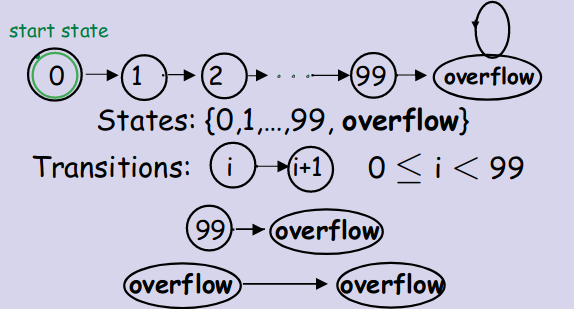
\includegraphics[width=0.9\textwidth]{../img/statemachine}
  \end{center}
\end{frame}

\subsection{Robot 1 Example}
\begin{frame}
  \frametitle{Example: Linear Robot 1.0}

  {\larger
    Imagine a robot that moves back and forth in a straight
    line. The robot has two speeds:

    \bigskip
    
    \begin{itemize}
    \item Forward, where it moves exactly \alert{five squares foward}.
    \item Back, where it moves exactly \alert{three squares back}.
    \end{itemize}

    \bigskip

    Starting from position {\bf 0}, is it possible for the robot to
    reach position 4?
  }  
\end{frame}

\begin{frame}
  \frametitle{Example: Linear Robot 1.1}
    {\larger
    Imagine a robot that moves back and forth in a straight
    line. The robot has two speeds:

    \bigskip
    
    \begin{itemize}
    \item Forward, where it moves exactly {\bf\alert{nine squares foward}.}
    \item Back, where it moves exactly \alert{three squares back}.
    \end{itemize}

    \bigskip

    Starting from position {\bf 0}, is it possible for the robot to
    reach position 4?

    \bigskip

    \structure{Why is it impossible for robot 1.1 reach square 4?}
  } 
\end{frame}

\begin{frame}
  \frametitle{Preserved Invariant States}

  {\larger
  \structure{Preserved Invariants} are variables in a state machine
  that are not modified by the actions of the computation steps.

  \bigskip

  {\bf Example:} The position of robot 1.1 is always $n+3k$ (n is the
  initial state, $k \in \mathbb{Z}$

  \bigskip
  
  Preserved Invariants can be used to perform induction on state
  machines:
  \begin{itemize}
    \item Prove that the preserved invariant, $P(s)$, holds for
      initial state $s_0$
    \item Prove that all transitions $P(s)$ to $P(s')$ do not change
      the invariant.
    \item Conclude that $P(s)$ holds for the entire computation. 
  \end{itemize}

  }
\end{frame}

\subsection{Robot 2 Example}

\begin{frame}
  \frametitle{Example 2: Diagonal Robot}

  {\larger
    Let's use invariants to prove or disprove the following:

    \bigskip

    Given a robot in $\mathbb{Z}^2$, that moves on the diagonals: (+1,
    +1), (-1,-1), (+1,-1), (-1,+1). Is it possible for the robot to
    reach position (1,0) from the initial position (0,0)?

    \begin{center}
      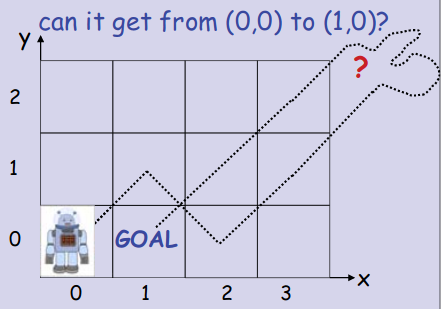
\includegraphics[width=0.6\textwidth]{../img/diag_robot}
    \end{center}
    
  }
\end{frame} 


\begin{frame}
  \frametitle{Example 2: Diagonal Robot}

  {\larger
  We can notice that one preserved invariant of the robot is that the
  sum of its coordinates is always even (or always odd):

  \bigskip
  \begin{itemize}
  \item P(0,0) is true (0+0 is even).
  \item The steps of the robot are:
    \begin{itemize}
    \item +1+1 = +2
    \item -1-1 = -2
    \item +1-1 = 0
    \item -1+1 = 0
    \end{itemize}
  \end{itemize}

  \bigskip

  From the steps/transitions. we see that if the sum of (x,y) is an
  oven number, any of the sucessor states will keep the same preserved
  invariant.
  
  }
\end{frame}

\begin{frame}
  \frametitle{Example 3: Fast Exponentiation}

  {\larger
    \begin{itemize}
    \item Please watch lecture video 1.9.1

      \bigskip
      
    \item To prove that an algorithm is correct, we need to prove two thngs:
      \begin{itemize}
      \item Prove that if the machine stops, the program is always
        correct (Correct output is a preserved invariant).
      \item Prove that the program halts at some point.  (follow an
        integer variable, and make sure that it decreases at every
        step)
      \end{itemize}
    \end{itemize}

    
  }
\end{frame}

%%%%%%%%%%%%%%%%%%%
% Chapter 1.10
% Recursive data type and structural induction
% Example with string bracket parsing.

% Structural Inductions for functions
% We can define a function based on structural induction
% We define the base case to hold
% And we define the constructors to hold as well.
% Examples:
% Function ``Depth'' of matching bracket strings
% Function ``Exponential'' that calculates fast exponentiation
%%%%%%%%%%%%%%%%%%%

%%%%%%%%%%%%%%%%%%%
% Read and maybe add 1.11
% Why are CS students interested in infinite sets? (computers are finite?)
% Well, we use infinite sets all the time, so we should
% be aware of it!
% The set of integers is infinite, the set of all matrixes is infinite, etc.
%
% The techniques used for measuring the size of infinite sets have profound
% Impacts on the logic of computation
%
% Infinite set sizes, countable sets, cantor's theorem
% Using Infinite sets to prove the Halting Problem
%%%%%%%%%%%%%%%%%%%%


% Make exercise questions
% Finish the set class above


\section{Conclusion}
\begin{frame}
  \frametitle{Extra Topics}

  {\larger
    \begin{itemize}
    \item Recusive Data Type and Structural Induction (1.10)

      \vfill
      
    \item Infinite Sets (1.11)
    \end{itemize}
  }
\end{frame}

\end{document}
